\documentclass{beamer}
\usepackage{pgfpages}
\usepackage[backend=bibtex]{biblatex}
\usepackage{multicol}
\usepackage{multimedia}
\usepackage[absolute,overlay]{textpos}
\usepackage{parskip}
\usepackage{hyperref}
\usepackage{lmodern}
\usepackage{caption}
\hypersetup{colorlinks=true, urlcolor=blue}
\setlength{\parskip}{\smallskipamount} 
%\usepackage[texcoord,grid,gridunit=mm,gridcolor=red!10,subgridcolor=green!10]{eso-pic} %DELETE when done with grid
\setbeameroption{hide notes} % Only slides
%\setbeameroption{show only notes} % Only notes
%\setbeameroption{show notes on second screen=right} % Both
%\bibliography{../../papers/references.bib}
\setbeamerfont{footnote}{size=\tiny}
%\AtEveryCitekey{\clearfield{title}}

%
% Choose how your presentation looks.
%
% For more themes, color themes and font themes, see:
% http://deic.uab.es/~iblanes/beamer_gallery/index_by_theme.html
%
\mode<presentation>
{
  \usetheme{Warsaw}      % or try Darmstadt, Madrid, Warsaw, ...
  \usecolortheme{default} % or try albatross, beaver, crane, ...
  \usefonttheme{default}  % or try serif, structurebold, ...
  \setbeamertemplate{navigation symbols}{}
  \setbeamertemplate{caption}[numbered]
} 

\usepackage[english]{babel}
%\usepackage[utf8x]{inputenc} %Doesn't play well with biblatex
\usepackage{amssymb}
\usepackage{bm}
\usepackage{color}
\usepackage{graphicx}

\newcommand{\red}[1]{{\color{red}{#1}}}

\title[{\color{white}{Day 5}}]{{\Huge Looking Ahead} \\ {\normalsize Clubes de Ciencia - Ensenada 2017 \\ Frank Wilzcek Course}}
\author{Cody Petrie \& David Rojas}
\institute{Universidad Aut\'onoma de Baja California}
\date{}
\titlegraphic{
\includegraphics[width=2cm]{../../logos/CdeC_logo.png}~%\hspace*{0.75cm}~
   
\includegraphics[width=1.5cm]{../../logos/UABC_logo.png}
}

\begin{document}

%\setbeamertemplate{frametitle}[default][center]
\begin{frame}
   \titlepage
\end{frame}

% Uncomment these lines for an automatically generated outline.
%\begin{frame}{Outline}
%  \tableofcontents
%\end{frame}

% Commands to include a figure:
%\begin{figure}
%\includegraphics[width=\textwidth]{your-figure's-file-name}
%\caption{\label{fig:your-figure}Caption goes here.}
%\end{figure}

\begin{frame}{Conventional Hyperspectral Applications}
   \begin{center}
      \Huge \textcolor{blue}{Conventional Hyperspectral Applications}
   \end{center}
\end{frame}

\begin{frame}{Hyperspectral Applications - Agriculture}
   \begin{center}
      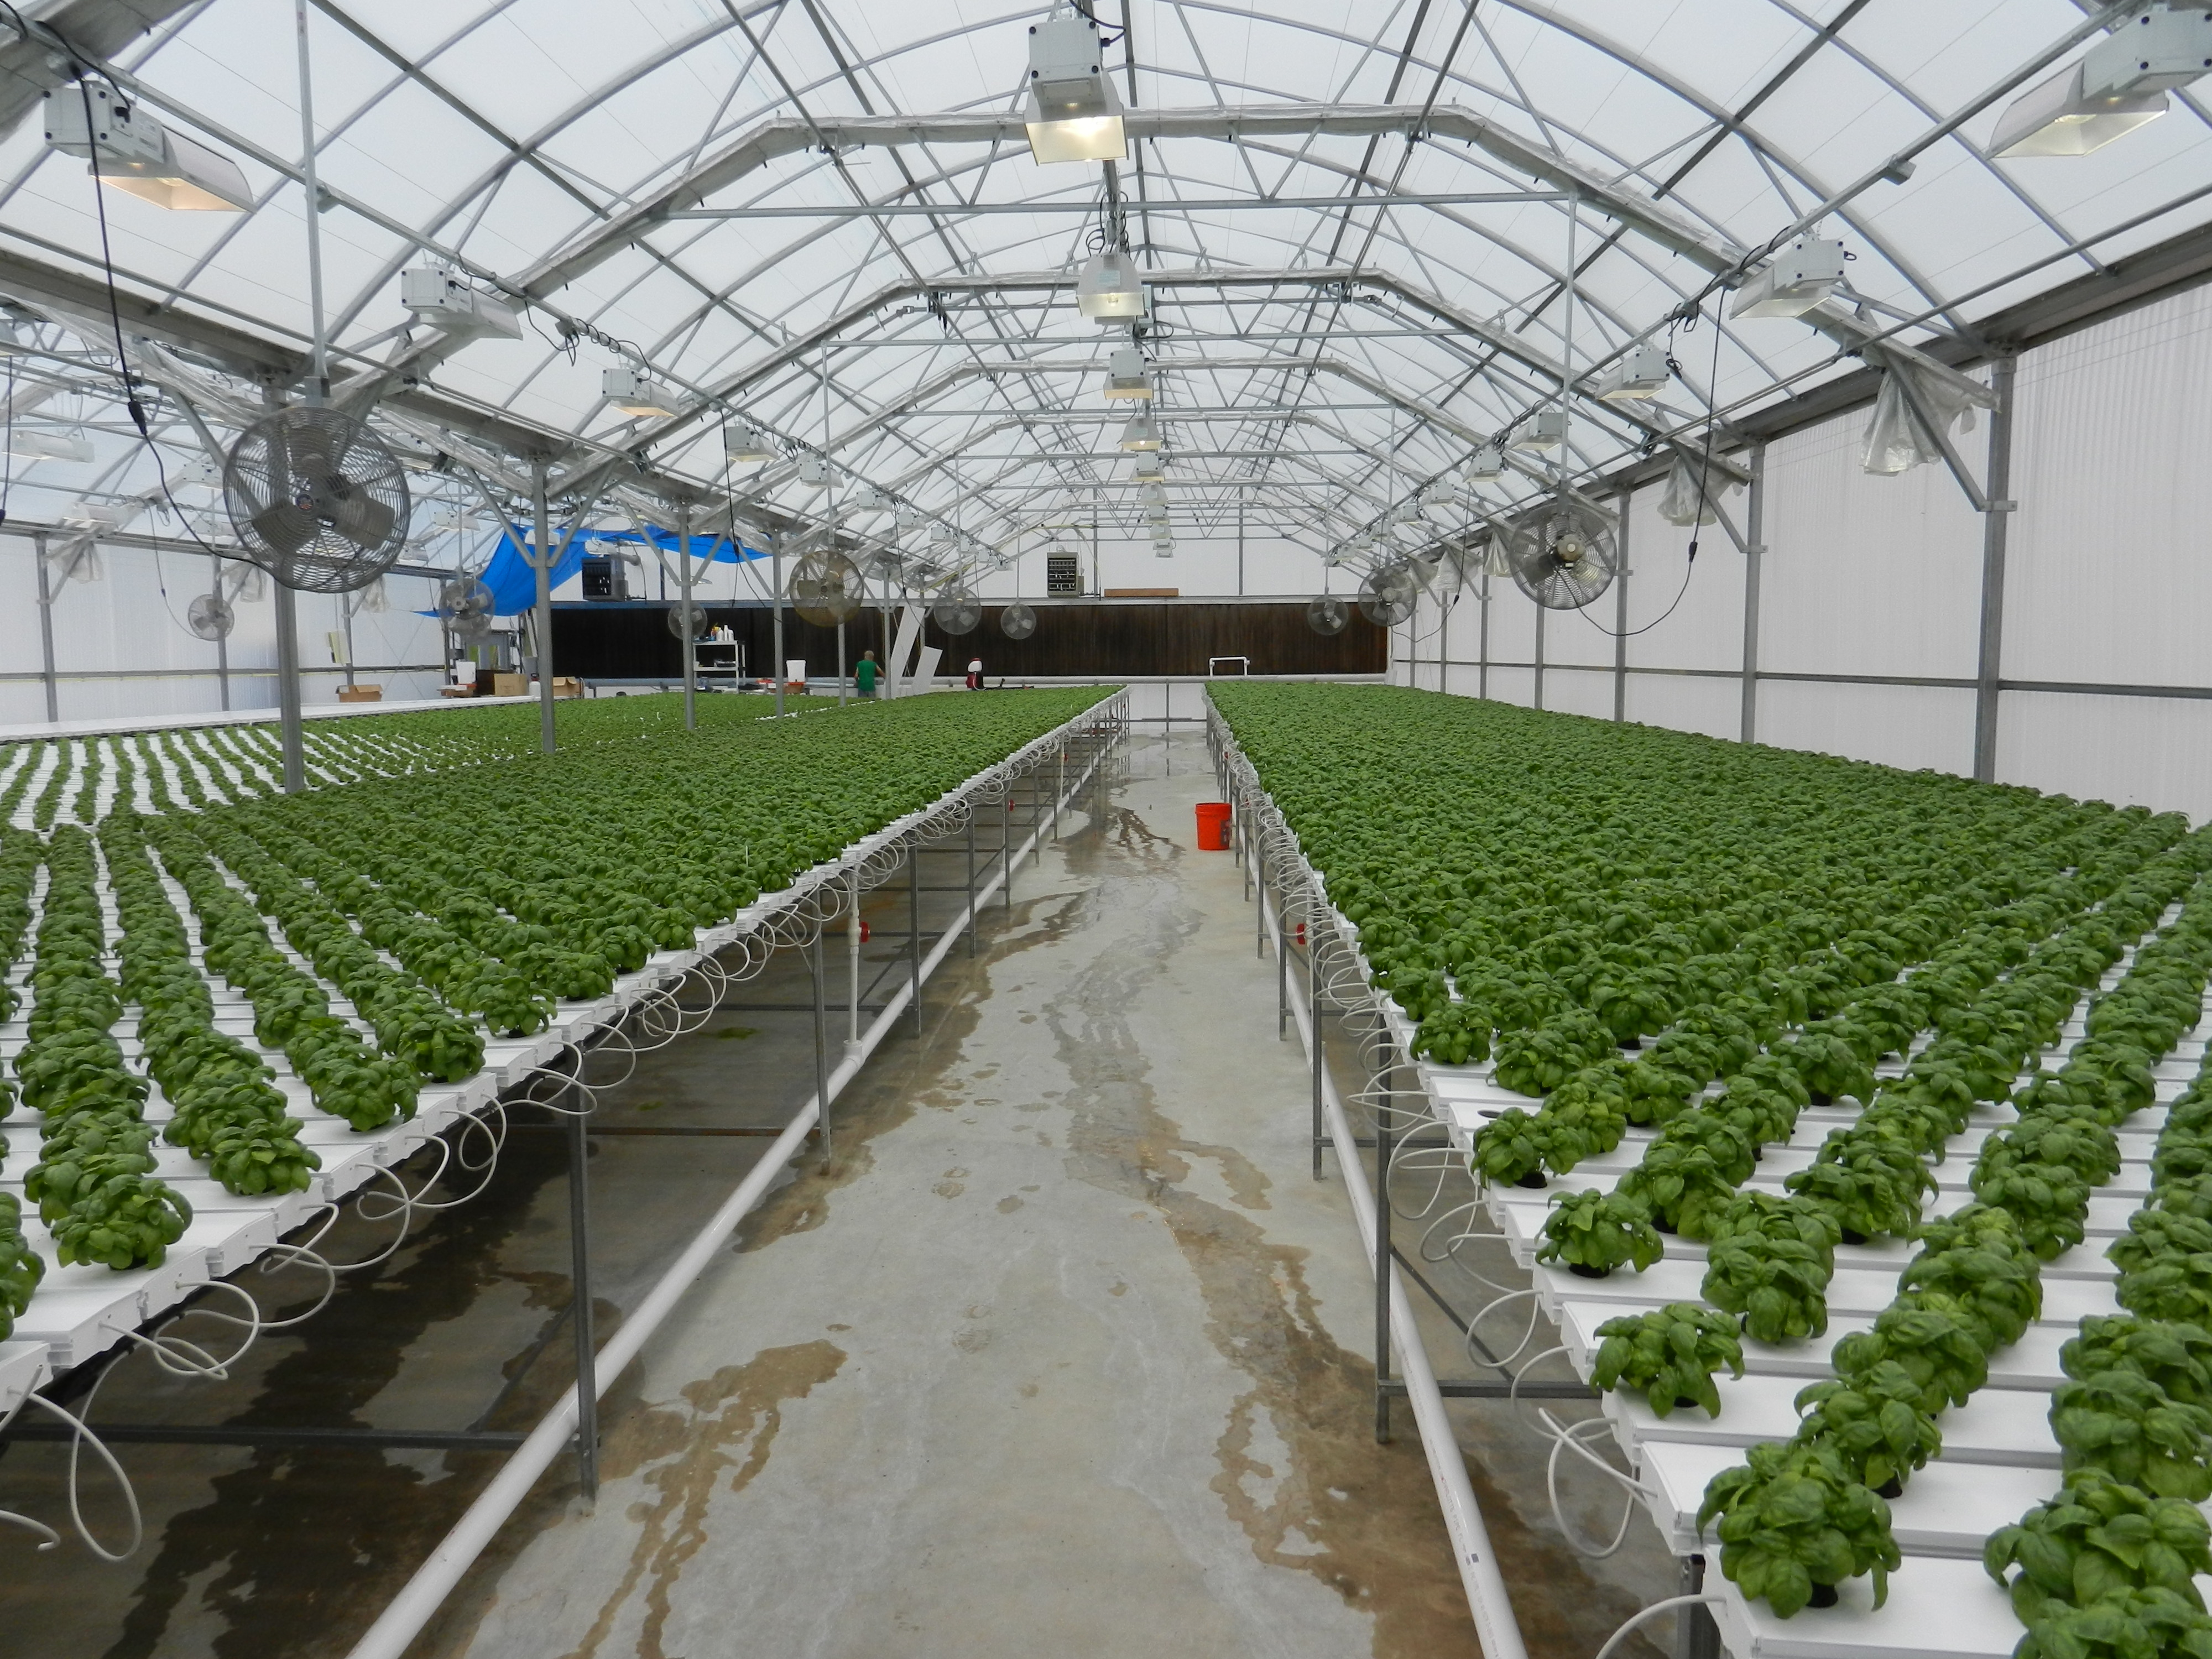
\includegraphics[width=0.8\textwidth]{figures/agriculture.jpg}
      \\Assessing plant health, monitoring ( + controlling?) light environment.
   \end{center}
\end{frame}

\begin{frame}{Hyperspectral Applications - Agriculture}
%   \begin{textblock*}{10cm}(0.3cm,1.5cm) % {block width} (coords)
   \begin{textblock*}{\textwidth}(0.05\textwidth,0.13\textwidth) % {block width} (coords)
      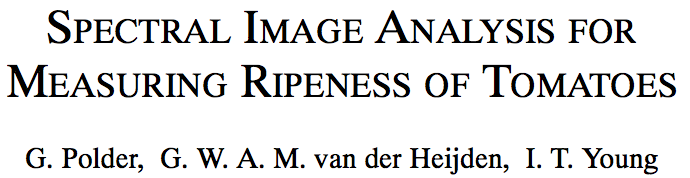
\includegraphics[width=0.4\textwidth]{figures/polder1.png}
   \end{textblock*}
   \begin{textblock*}{10cm}(0.4cm,3.0cm) % {block width} (coords)
      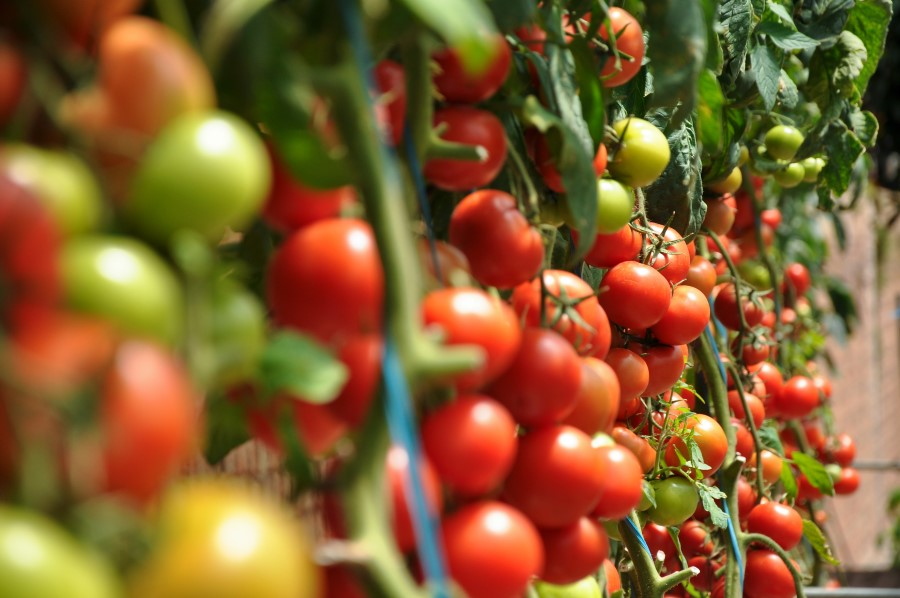
\includegraphics[width=4.5cm]{figures/tomatoes.jpg}
      \\ Wavelengths used: 396-736 nm
   \end{textblock*}
   \begin{textblock*}{10cm}(5.5cm,1.5cm) % {block width} (coords)
      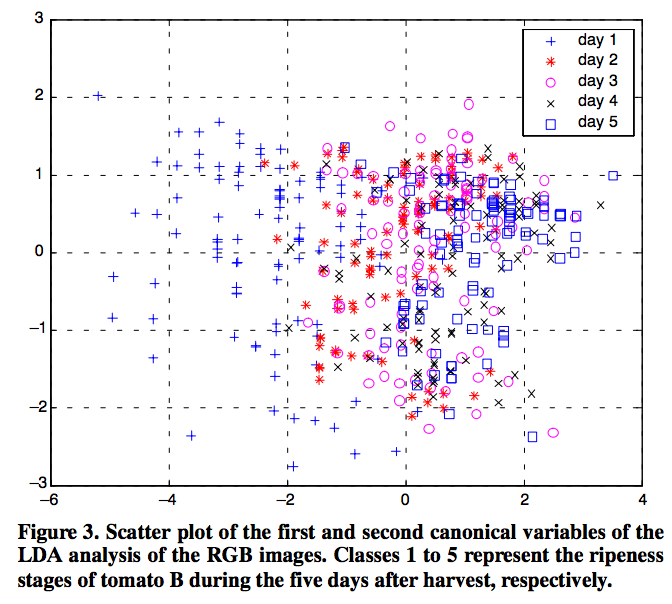
\includegraphics[width=4cm]{figures/polder2.png}
   \end{textblock*}
   \begin{textblock*}{\textwidth}(5.5cm,2.5cm) % {block width} (coords)
      \begin{center}
         {\huge Consumer \\ Camera} \\ {\Huge $\leftarrow$}
      \end{center}
   \end{textblock*}
   \begin{textblock*}{10cm}(8.6cm,5.3cm) % {block width} (coords)
      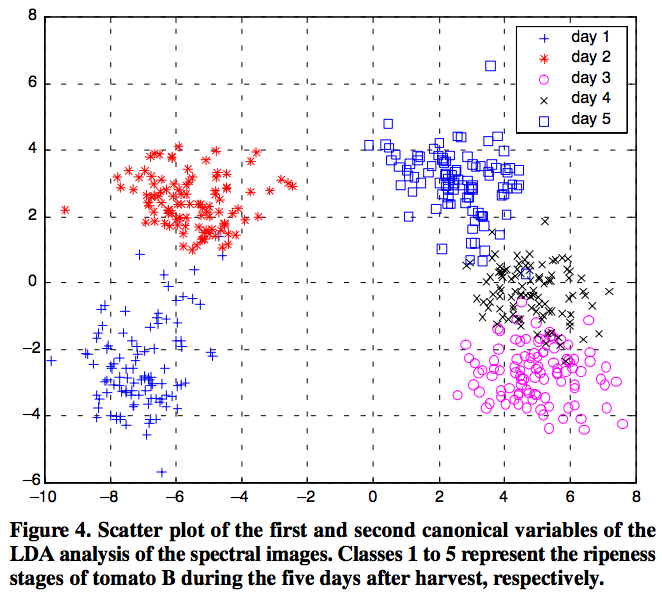
\includegraphics[width=4cm]{figures/polder3.png}
   \end{textblock*}
   \begin{textblock*}{\textwidth}(1.3cm,6.5cm) % {block width} (coords)
      \begin{center}
         {\huge Hyperspectral \\ Camera} \\ {\Huge $\rightarrow$}
      \end{center}
   \end{textblock*}
\end{frame}

\begin{frame}{Hyperspectral Applications - Art and Archaeology}
   \begin{center}
      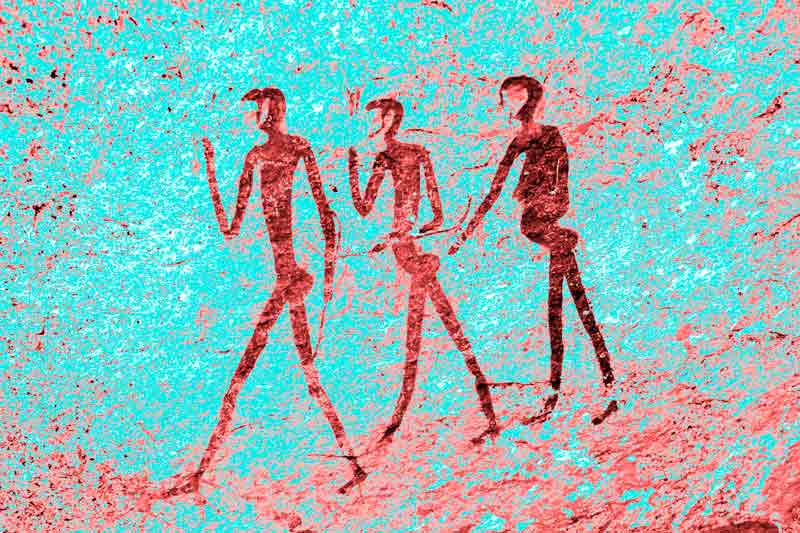
\includegraphics[width=0.8\textwidth]{figures/archaeology.jpg}
      \\Determining the nature of pigments and materials, finding under-paintings.
   \end{center}
\end{frame}

\begin{frame}{Hyperspectral Applications - Biology}
   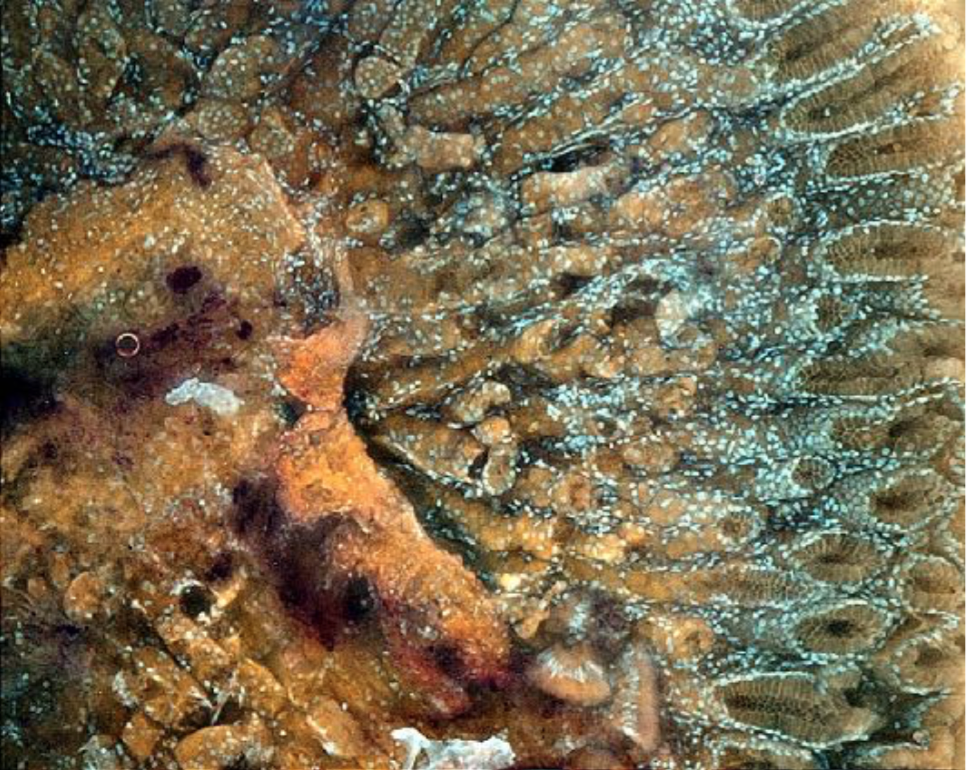
\includegraphics[width=0.8\textwidth]{figures/colon.png}
   \begin{textblock*}{\textwidth}(5.7cm,3.5cm) % {block width} (coords)
      \begin{center}
         \color{red}{MUSE \\(Microscopy \\with UV Surface \\Enhancement) \\image of colon}
      \end{center}
   \end{textblock*}
   \begin{center}
      Determining the absorption patterns of dyes, notably including fluorescent proteins.
   \end{center}
\end{frame}

\begin{frame}{Hyperspectral Applications - Food}
   \begin{center}
      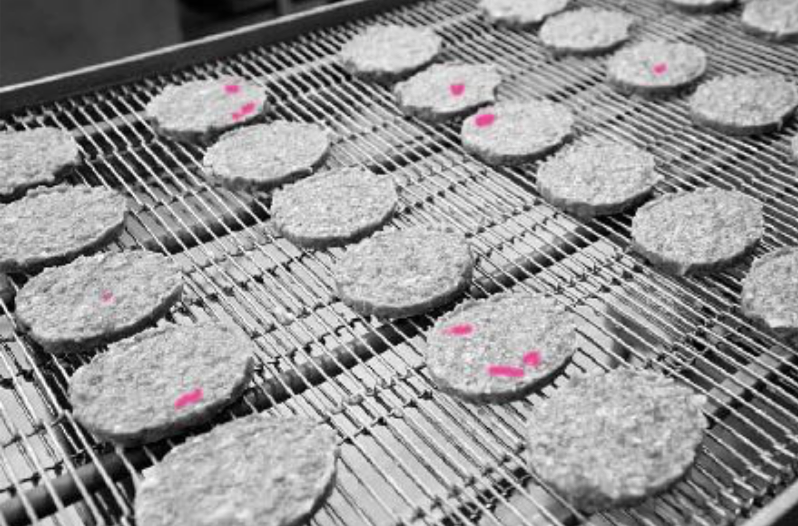
\includegraphics[width=0.8\textwidth]{figures/hamburger.png}
      \\Inspecting food sanitation before being sent to the consumer.
   \end{center}
\end{frame}

\begin{frame}{Hyperspectral Applications - Forensics}
   \begin{center}
      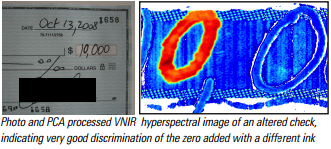
\includegraphics[width=\textwidth]{figures/forensics.png}
      \\~\\Finding faulty checks or other (bio) markers that could be used as evidence.
   \end{center}
\end{frame}

\begin{frame}{Hyperspectral Applications}
   \begin{itemize}
      \item There are also opportunities for artistic creation and display.
      \item For example, how about movies showing:
      \begin{itemize}
         \item Hyperspectral sunrises, sunsets and fireworks?
         \item Hyperspectral rainbows (and multi-rainbows)?
      \end{itemize}
      \item Or how about routinely experiencing the world - or an art museum, or virtual reality - in an enhanced way, through appropriate goggles, smartphone display, or illumination?
   \end{itemize}
\end{frame}

\begin{frame}{Hyperspectral Applications}
   \begin{itemize}
      \item "I can't escape the feeling that the best ideas are yet to come." - Frank Wilczek
      \item "Those ideas may/will come from YOU guys!" - Me :)
   \end{itemize}
\end{frame}

\begin{frame}{Other Encodings}
   \begin{itemize}
      \item This course has mainly focused on vision and hearing, but there are many other ways of sensing the world.
      \item In your future explorations, for example in designing useful devices or understanding animal behavior, you might want to think about other sensory possibilities.
      \item For example \ldots
   \end{itemize}
\end{frame}

\begin{frame}{Other Encodings}
   \begin{itemize}
      \item The ``North Paw" sensor vibrates when you’re facing north. (This device caught Frank's imagination, and first got him thinking about enhanced perception ... )
      \begin{center}
         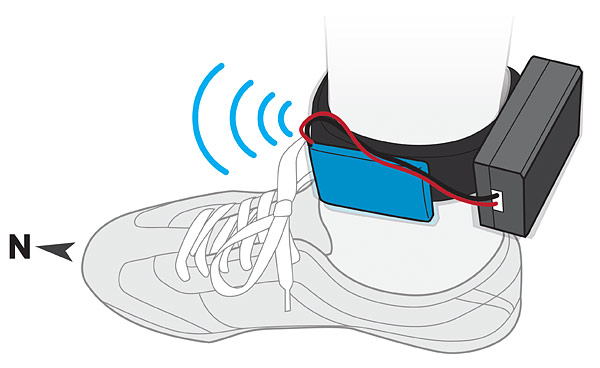
\includegraphics[width=0.8\textwidth]{figures/northpaw.jpg}
      \end{center}
      \item People have also ``restored" a weak form of vision to blind people in this way.
   \end{itemize}
\end{frame}

\begin{frame}{Other Encodings}
   \begin{itemize}
      \item Smell and taste are chemical senses. Roughly speaking, their receptors key in on shapes of molecules.
      \item One can design digital chemical sensor arrays, with visual (or audible) output. There are many options for what is sensed, and how to display it.
      \begin{center}
         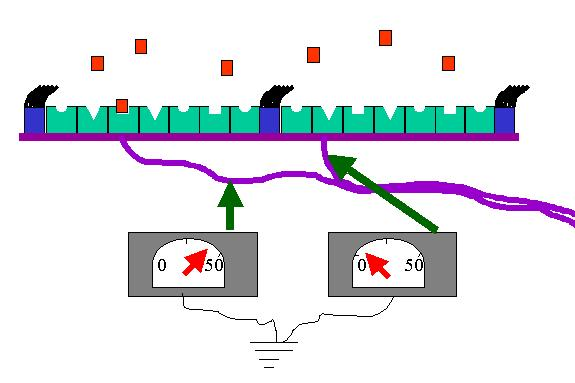
\includegraphics[width=0.45\textwidth]{figures/noseshapes.jpg}
         ~ 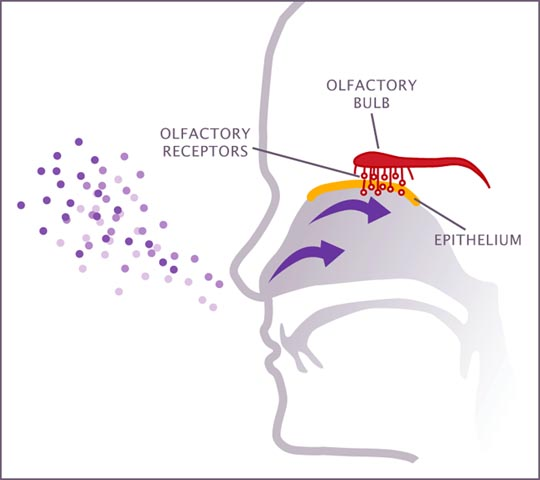
\includegraphics[width=0.45\textwidth]{figures/smell.jpg}
      \end{center}
   \end{itemize}
\end{frame}

\begin{frame}{Other Encodings}
   \begin{center}
      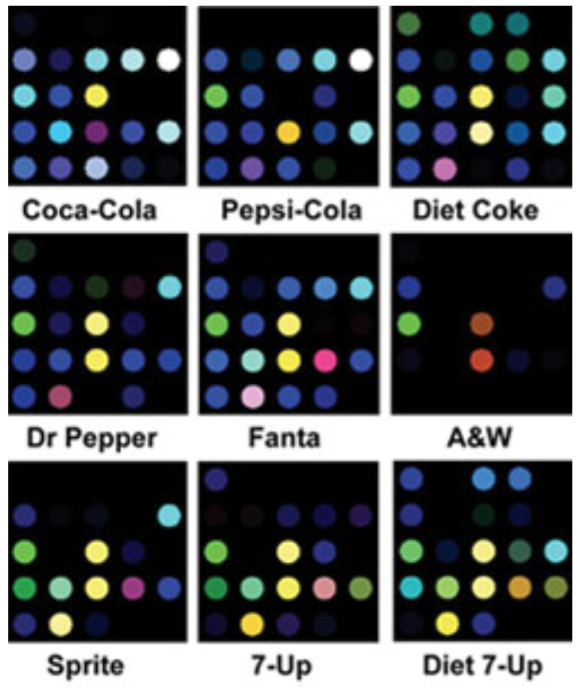
\includegraphics[width=0.5\textwidth]{figures/sodapop.png}
      \\Outputs from an artificial chemical sensor array
   \end{center}
\end{frame}

\begin{frame}{Other Encodings}
   \begin{itemize}
      \item This design accommodates a combinatorial explosion: with $M$ locations, each allowing $k$ colors, we have $k^M$ possible patterns.
      \item With $k = 2$ (on/off) and $M = 24$, we have over 16 million possibilities.
      \item Note that patterns that have a lot in common represent things that have a lot in common, encouraging associative memory.
   \end{itemize}
\end{frame}

\begin{frame}{Other Encodings}
   \begin{itemize}
      \item Other possible sensory modalities include: force-detectors and motion-detectors
      \begin{itemize}
         \item Pressure and vibration detectors
         \item Temperature detectors (including infrared vision)
         \item Electric and magnetic field detectors
      \end{itemize}
      \item Any of these might be built into remote sensors, or robots.
      \begin{center}
         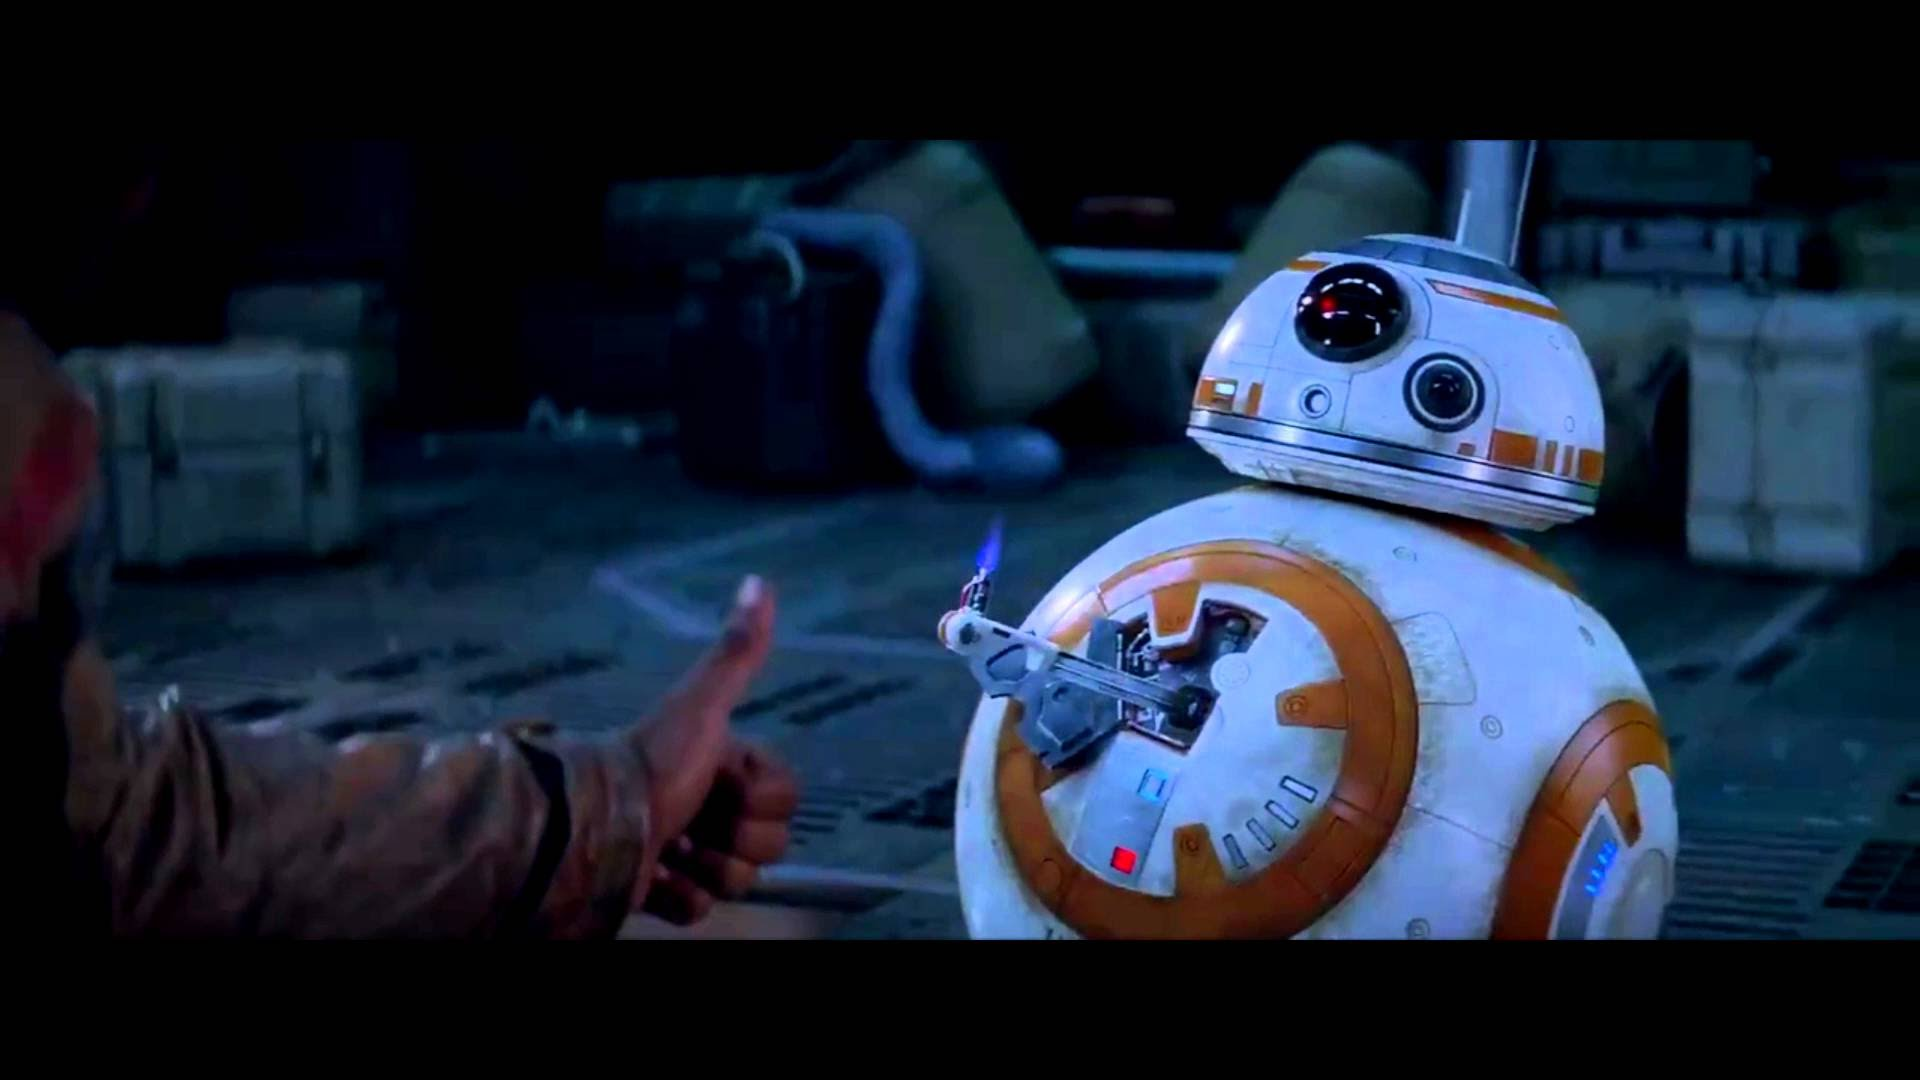
\includegraphics[width=0.5\textwidth]{figures/bb8.jpg}
      \end{center}
      \item Then an issue is how to present the information to humans, whose most capable portals are visual (especially) and aural.
      \item Our tricks can be helpful in that regard!
   \end{itemize}
\end{frame}

\begin{frame}{Summary and Conclusion}
   \begin{center}
      \Huge \textcolor{blue}{Summary and Conclusion}
   \end{center}
\end{frame}

\begin{frame}{Summary and Conclusion}
   \begin{itemize}
      \item There's a lot more ``out there" than we ordinarily perceive.
      \item Modern technology is opening up important opportunities to perceive more, which can be fun, useful, and not necessarily expensive or impractical.
      \item We've tried to give you some tools to think intelligently - and creatively - about those opportunities.
      ~\\~\\
   \end{itemize}
   \begin{center}
      {\Huge Now go make the world a better place!}
   \end{center}
\end{frame}

\begin{frame}{Picture Citations} 
\fontsize{5}{4}\selectfont  
CdeC logo (accessed 13 July 2017): \href{https://www.clubesdeciencia.mx}{https://www.clubesdeciencia.mx}\\
UABC logo (accessed 13 July 2017): \href{http://www.uabc.mx/}{http://www.uabc.mx/}\\
Agriculture (accessed 19 July 2017): \href{http://www.nexuscorp.com/controlled.asp}{http://www.nexuscorp.com/controlled.asp}\\
Tomatoes (accessed 19 July 2017): \href{http://wonderopolis.org/wp-content/uploads/2016/04/dreamstime\_xl\_20359776\_(Custom).jpg}{http://wonderopolis.org/wp-content/uploads/2016/04/dreamstime\_xl\_20359776\_(Custom).jpg}\\
Wall painting (accessed 19 July 2017): \href{http://aeronics.in/distribution/multispectral\_camera}{http://aeronics.in/distribution/multispectral\_camera}\\
Check Fraud (accessed 19 July 2017): \href{http://www.middletonspectral.com/applications/other-applications/forensics/}{http://www.middletonspectral.com/applications/other-applications/forensics/}\\
North paw (accessed 21 July 2017): \href{http://www.thinkgeek.com/product/f358/}{http://www.thinkgeek.com/product/f358/}\\
Smell with shapes (accessed 21 July 2017): \href{https://aqfi.uaex.edu/people/faculty/akelly/z-agoodwin-and-files/Web-Files/Delete/BIOF\%20Web\%20page\%202011/Text/12\%20taste\%20and\%20smell/Tastsm15.htm}{https://aqfi.uaex.edu/people/faculty/akelly/z-agoodwin-and-files/Web-Files/Delete/BIOF\%20Web\%20page\%202011/Text/12\%20taste\%20and\%20smell/Tastsm15.htm}\\
Nose (accessed 21 July 2017): \href{http://easyscienceforkids.com/whats-that-smell-all-about-your-sense-of-smell/}{http://easyscienceforkids.com/whats-that-smell-all-about-your-sense-of-smell/}\\
BB8 (accessed 21 July 2017): \href{https://i.ytimg.com/vi/\_RWWKFqv7EM/maxresdefault.jpg}{https://i.ytimg.com/vi/\_RWWKFqv7EM/maxresdefault.jpg}\\
\end{frame}

\end{document}
